\documentclass{beamer}
\usepackage[T1]{fontenc}
\usepackage{textcomp}
\usepackage[utf8]{inputenc} %per riuscire a scrivere gli accenti
\usepackage[italian]{babel} % lingua del documento
\usepackage{url} % per scrivere gli indirizzi Internet

\usepackage{amssymb,amsmath,amsthm,amsfonts}
%\usepackage{multimedia}
%COMANDI%%%%%%%%%%%%%%%%%%%%%%%
\usepackage[qm]{qcircuit}


\newcommand{\bra}[1]{\left\langle #1 \right |}
\newcommand{\ket}[1]{\left| #1 \right \rangle}
\newcommand{\braket}[2]{\left\langle #1 | #2 \right\rangle}

\renewcommand{\d}[0]{\mathrm{d}}
%ROCCO%
%\newcommand{\dd}[0]{\mathrm{d}}


\newcommand{\vmed}[1]{\left \langle #1 \right \rangle}
\newcommand{\vmedvec}[1]{\langle #1 \rangle}
\newcommand{\abs}[1]{\left| #1 \right|}
\newcommand{\R}[0]{\mathbb{R}}
\newcommand{\absvec}[1]{| #1 |}
\newcommand{\norm}[1]{{\left|\!\left| #1 \right|\!\right|}}
\newcommand{\normvec}[1]{|\!| #1 |\!|}
\newcommand{\tr}{\operatorname{Tr}}
\newcommand{\dev}[2]{\displaystyle \frac{\d #1}{\d #2}}
\renewcommand{\H}[0]{\operatorname{H}}
\renewcommand{\Re}[1]{\operatorname{\mathbb{R}e}\left[ #1 \right]}
\renewcommand{\Im}[1]{\operatorname{\mathbb{I}m}\left[ #1 \right]}



\newcommand{\ketbra}[2]{| #1 \rangle \langle #2 |}
\newcommand{\F}[0]{\mathcal{F}}
\renewcommand{\O}[0]{\mathcal{O}}
\newcommand{\E}[0]{\mathcal{E}}
\renewcommand{\epsilon}[0]{\varepsilon}
\renewcommand{\'}[0]{\`}

%Tabelleeeeeeee
\usepackage{booktabs}
\usepackage{caption}
\usepackage{graphicx}
\usepackage{color, colortbl}
\definecolor{Gray}{gray}{0.9}
\usepackage{array}





\usetheme{Padova}

\title{Quantum computing programming languages}

\author
{
\parbox[t]{2cm}{Laureanda:} \textbf{Alice Pagano}\\
\parbox[t]{2cm}{Relatore:} \textbf{Prof. Simone Montangero}
}
\date
{
\vspace{2mm}
24 Settembre 2019
}

%\AtBeginSection[]
%{
%  \begin{frame}
%    \frametitle{Indice}
%    \tableofcontents[currentsection]
%  \end{frame}
%}


%Backupp!!!!

\newcommand{\backupbegin}{
   \newcounter{finalframe}
   \setcounter{finalframe}{\value{framenumber}}
}
\newcommand{\backupend}{
   \setcounter{framenumber}{\value{finalframe}}
}


\begin{document}

	\maketitle

	\section{Introduzione}
	
	
	
	\begin{frame}{Quantum computing: che cos'è?}
	
	\begin{figure}[h!]
	\begin{columns}
 
	\column{0.5\textwidth}
	\centering \includegraphics[width=0.7\textwidth]{./tikz/Classical.pdf}
	
	\column{0.5\textwidth}
	\centering \includegraphics[width=0.7\textwidth]{./tikz/Quantum.pdf}
	\end{columns}
	\end{figure}

	\end{frame}
		
	\begin{frame}{Quantum computing: che cos'è?}
	
	\begin{alertblock}{Qual è la differenza?}
	Fenomeni quantistici, come l'\alert{entanglement}, rendono l'informazione processata da un sistema quantistico molto diversa da quella di un computer classico. \pause	
	\end{alertblock}
	
	\vspace{1cm}
	
	\begin{alertblock}{A cosa serve un computer quantistico?}
	Risolvere problemi impossibili da risolvere con un computer classico per via del grande \alert{costo computazionale}. 
	\end{alertblock}
	
	
	
	
	\end{frame}

		
	
	
%	\begin{frame}{Indice}
%		\tableofcontents
%	\end{frame}


\section{Concetti fondamentali}

	\begin{frame}{Qubit}

	\begin{columns}
 
	\column{0.6\textwidth}
	
	\pause
	
	Un qubit è un sistema quantistico a due livelli. \pause
	\vspace{0.5cm}
	
	Genericamente, il suo stato si può scrivere come una combinazione lineare degli stati $ \ket{0} = \begin{pmatrix} 1 \\ 0 \end{pmatrix} $ e $\ket{1} = \begin{pmatrix} 0 \\ 1 \end{pmatrix}  $: 
	
	\vspace{0.1cm}
	\begin{equation*}
  	% \begin{gathered}	
 	\ket{\psi}= \cos{ \frac{\theta}{2}} \ket{0} + e^{i \phi} \sin{ \frac{\theta}{2}} \ket{1} 
  	% \end{gathered}	
	\end{equation*}
	\vspace{0.1cm}
		
	dove $ 0\leq \theta \leq \pi$, $0\leq \phi < 2\pi$. 

	
	\column{0.4\textwidth}
	\begin{figure}
	\centering \includegraphics[width=1\textwidth]{./tikz/BlochSphere.pdf}
	\caption{Sfera di Bloch.}
	\end{figure}
	\end{columns}
	

	\end{frame}

	
	\begin{frame}{Matrice densità}
	
	\begin{block}{Stato puro}
	Stato di informazione massimale. 
	\end{block}
	\begin{block}{Stato misto}
	Stato di informazione non massimale. 	
	\end{block}
	
	\begin{alertblock}{Matrice densità}
	Consideriamo un sistema che si trova nello stato $\ket{\psi_i}$ con probabilità $p_i$.
	La matrice densità è definita come 
	\begin{equation*}
	 \rho = \sum_i p_i \ket{\psi_i}\bra{\psi_i} 
	 \end{equation*}
	\end{alertblock}
	

	\end{frame}

	

	\begin{frame}{Entanglement}
	
	\'E un fenomeno \alert{puramente quantistico}, che implica una correlazione intrinseca tra i costituenti del sistema. 
	\vspace{0.3cm}
	
	Matematicamente, uno stato entangled \alert{non} può essere fattorizzato come il prodotto tensore degli stati costituenti: 	
	\begin{equation*}
	(\rho^{AB}) = \sum_i p_i (\rho_i^A \otimes \rho_i^B).
	\end{equation*} \pause
	
	\vspace{-0.5cm}
	\begin{exampleblock}{Stato GHZ}
	Per un sistema con $N>2$ qubit, si definisce:
	\begin{equation*}
	\ket{\text{GHZ}}= \frac{\, \, \ket{0}^{\otimes N} + \ket{1}^{\otimes N} }{\sqrt{2} }
	\end{equation*}
	\end{exampleblock}	
	
	\end{frame}

	\begin{frame}{Quantum gate}
	Un circuito quantistico di $n$-qubit è costituito da:
	
	\[ 
\Qcircuit @C=1.6em @R=1.2em {
& & &\lstick{\ket{0}} & \qw & \multigate{3}{\hat{U_1}} & \qw & \gate{\hat{U_2}}  & \qw & \meter \\
n & & & \lstick{\ket{0}} & \qw & \ghost{\hat{U_1}} & \qw & \qw & \qw & \meter \\
qubits & & & \lstick{ \vdots \ }& \cdots & \nghost{\hat{U_1}} & \cdots & \cdots  & \cdots & \vdots \\
& & & \lstick{\ket{0}}& \qw &  \ghost{U_1} & \gate{\hat{U_3}} & \qw & \qw & \meter
%\inputgroupv{1}{4}{2.8em}{2.8em}{ }
\gategroup{1}{3}{4}{3}{2.3em}{\{}
}
 \]
  \pause
 	I gate quantistici sono rappresentati da \alert{matrici unitarie} $\hat{U}$. L'azione di un gate si può rappresentare come:
	
	
	\begin{equation*}
 	\ket{\psi'}= \hat{U} \ket{\psi}
	\end{equation*} 
	
	\end{frame}
	
	\begin{frame}{Quantum gate}
	\vspace{-0.4cm}
	
	\begin{exampleblock}{Hadamard gate}
	\begin{equation*}
H= \frac{1}{\sqrt{2}}
\begin{pmatrix}
1 & 1 \\
1 & -1
\end{pmatrix} \hspace{1cm}
\Qcircuit @C=1em @R=.7em {
&\qw & \gate{H} & \qw & \qw
}  
\label{HGate}
\end{equation*}
\small{Crea una sovrapposizione degli stati $\ket{0}$ e $\ket{1}$.}
	\end{exampleblock} \pause

	\begin{exampleblock}{Controlled-X gate}
\begin{equation*}
 C_X = 
\begin{pmatrix}
1 & 0 & 0 & 0\\
0 & 1 &0 &0\\
0 &0 & 0 & 1\\
0 &0 &1 &0
\end{pmatrix} \hspace{1cm}
 \Qcircuit @C=1em @R=1.2em {
& \qw &\ctrl{1} & \qw & \qw \\
& \qw & \targ  & \qw & \qw
}  
\end{equation*}
\small{Inverte lo stato del qubit bersaglio se il qubit controllore è nello stato $\ket{1}$.}
	\end{exampleblock}
	
		
	\end{frame}

		
	\begin{frame}{Quantum channel}	
	Un sistema che interagisce con un \alert{ambiente esterno} è affetto durante la sua dinamica da rumore. \pause
	
	\vspace{0.5cm}
	Il rumore quantistico può essere riprodotto introducendo un set di \alert{canali quantistici} che agiscono come:
	
	\begin{equation*}
	 \rho \rightarrow \rho ' =  \sum_k E_k \rho E_k^\dagger
	 \end{equation*} 
	

	
	\end{frame}

	\begin{frame}{Quantum channel}	
	
	\small I canali a \alert{singolo qubit} possono essere illustrati da una trasformazione affine che trasforma la sfera di Bloch in un ellissoide con volume minore o uguale. 
	\vspace{0.4cm}
					
	\begin{columns}
		
	\column{0.5\textwidth}
	\centering \includegraphics[width=0.7\textwidth]{./image/depolarizing.eps}
	
	\column{0.5\textwidth}
	\centering \includegraphics[width=0.7\textwidth]{./image/amplitudedamping.eps}	
	
	\end{columns}
	
	\vspace{0.3cm} \pause
	
	\centering $\longrightarrow$ Tempi di rilassamento
	
	\end{frame}
					
\section{Quantum computer: software}

\setbeamercovered{dynamic} 	
	
	\begin{frame}{Quantum software: Qiskit e Cirq}

	Il software quantistico si occupa della comunicazione con un device
	 Il linguaggio di programmazione usato è \alert{Python}.  \pause

	\vspace{0.5cm}

	%\begin{columns}
%	\hspace{-0.5cm}



\centering
\only <1> { \includegraphics[width=0.9\textwidth]{./image/Schema1.png}} 
\only <2-> { \includegraphics[width=0.9\textwidth]{./image/Schema2.png}} 



%	\begin{figure}
%	 \includegraphics[width=0.9\textwidth]{./image/Schema2.png} 
%	\end{figure}

		
	%\centering \includegraphics[width=0.9\textwidth]{./image/Schema2.png} 
		
%	\column{0.35\textwidth}
%	
%	\centering \includegraphics[width=0.35\textwidth]{./image/Qiskit.png} \\
%	\centering \small Qiskit (IBM software) \\
%	\vspace{0.5cm}
%	
%	\centering \includegraphics[width=0.5\textwidth]{./image/Cirq.png}  \\ 
%	
%	\centering{ \small Cirq (Google software)}	\pause
%	
%	
%	\column{0.65\textwidth}
%	\strut \vspace*{-\baselineskip}
%		\strut \vspace*{-\baselineskip}
%		\strut \vspace*{-\baselineskip}		
%\begin{center}	
%\begin{tabular}[t]{ |p{3.7cm}| p{1cm}| p{1cm}|  }
%\toprule
%& Qiskit & Cirq  \\
%\midrule
%\rowcolor{Gray}
%Simulatori &  \includegraphics[width=0.05\textwidth]{./image/vero.png}  & \includegraphics[width=0.05\textwidth]{./image/vero.png} \\
%Quantum computer &  \includegraphics[width=0.05\textwidth]{./image/vero.png}   & \includegraphics[width=0.05\textwidth]{./image/falso.png}  \\
%\rowcolor{Gray}
%Circuito parametrizzato  &  \includegraphics[width=0.05\textwidth]{./image/vero.png} &   \includegraphics[width=0.05\textwidth]{./image/vero.png} \\
%Noise model & \includegraphics[width=0.05\textwidth]{./image/vero.png}  & \includegraphics[width=0.05\textwidth]{./image/falso.png}\\
%\rowcolor{Gray}
%Community  &   \includegraphics[width=0.05\textwidth]{./image/vero.png}    & \includegraphics[width=0.05\textwidth]{./image/falso.png}  \\
%\bottomrule
%\end{tabular}	
%\end{center}


%	\end{columns}


	
 	\end{frame}

\setbeamercovered{} 


	\begin{frame}{IBM Q Melbourne}
	\alert{IBM Q Melbourne}: quantum computer con $n=\alert{14}$ qubit. \pause
	\vspace{0.5cm}
	
	\begin{figure} \includegraphics[width=1\textwidth]{./tikz/IBMQMelbourne.pdf} \caption{Mappa di accoppiamento di IBM Q Melbourne. } \end{figure}
	 \vspace{0.5cm}
	 
	\end{frame}
	
	
			
\section{Verifica di stati GHZ}
	
	\begin{frame}{Verifica di stati GHZ}
	
	\alert{OBIETTIVO}: misura bontà stato GHZ $\rightarrow$  fidelity.
	
	\hspace{6.7cm} $\text{F}= | \braket{\psi_0}{\psi (t)} |^2 $  \pause
	\vspace{0.5cm}
	
	\alert{ESPERIMENTO}: 
	\begin{itemize}
	\item In uno stato GHZ \alert{\textit{ideale}}, se ciascun qubit ha una rotazione di fase $\phi$, allora $N$-qubit ruotano collettivamente di $N\phi$. 
	\item In presenza di \alert{rumore}, lo stato GHZ è parzialmente misto e una fase differente può essere osservata.
	\end{itemize}
	
	
	 Osservando come uno stato GHZ \textit{non ideale} risponde a rotazioni di fase, è possibile vincolare la fidelity dello stato $\rightarrow$ misura di MQC (\alert{Multiple Quantum Coherence}).



	\end{frame}
	
	\begin{frame}{Circuito MQC}
	
	\begin{center}

\[ 
\Qcircuit @C=1.2em @R=0.7em {
\lstick{\ket{0}} & \gate{H} & \multigate{3}{U_{CX}} &  \gate{U_{\phi}}& \multigate{3}{U_{CX}^{\dagger}} & \gate{H}  & \meter \\
 \lstick{\ket{0}} & \qw & \ghost{U_{CX}}  & \gate{U_{\phi}} & \ghost{U_{CX}^{\dagger}} & \qw &  \meter \\
 \lstick{ \vdots \ }& \qw & \ghost{U_{CX}} & \gate{U_{\phi}} & \ghost{U_{CX}^{\dagger}} & \qw  &  \meter \\
 \lstick{\ket{0}}& \qw &  \ghost{U_{CX}} &  \gate{U_{\phi}} & \ghost{U_{CX}^{\dagger}} &\qw & \meter
}
 \]
 
 \captionof{figure}{Circuito MQC per $N$ qubit con $U_{\phi} =  \begin{pmatrix} e^{- i \frac{\phi}{2} } & 0 \\ 0 & e^{ i \frac{\phi}{2} } \end{pmatrix}  $.}

\end{center}
	
	\end{frame}
	
	
	\begin{frame}{Misura}

Il circuito MQC di \alert{$N$} qubit è stato implementato nei due software. \pause
\vspace{0.5cm}


Il processo di misura è stato eseguito nel seguente modo: \pause

\begin{enumerate}
\item si è fissato il valore di \alert{$\phi$} e il circuito è stato eseguito in un device.  \pause
\item si è misurata  la fase amplificata, calcolando la probabilità che il sistema ritorni nello stato iniziale,  \alert{$ S_{\phi}$}. \pause
\item gli step 1-2 sono eseguiti nuovamente per ciascun valore di $\phi_j = \frac{ \pi j }{N+1}$, dove $j=0,1,2,\dots,2N+1$. 

Si è così ottenuta una lista di misure per \alert{differenti} valori di $\phi$.

\end{enumerate}

	\end{frame}
	
	\begin{frame}{Analisi: ampiezze MQC}

L'analisi è stata eseguita nel seguente modo: \pause

\begin{enumerate}
\item si sono illustrati in uno stesso grafico \alert{$ S_{\phi}$} e \alert{$ S_{\phi}^{ideale}$}. \pause
\item si sono calcolate per $ S_{\phi}$ e $ S_{\phi}^{ideale}$ le \alert{ampiezze MQC}, definite come
 \begin{equation*}
I_{q}= \mathcal{N}^{-1} | \sum_{\phi} e^{i q \phi} S_{\phi} | 
\end{equation*} 
e sono calcolate tra $[-N,N]$. \pause
\item Infine, si è limitata la \alert{fidelity} dello stato: 
\begin{equation*}
 2 \sqrt{I_N} \leq F \leq \sqrt{I_0/2} + \sqrt{I_N}
 \label{Fidelity_Bounded}
 \end{equation*}

\end{enumerate}


	
	\end{frame}

	\begin{frame}{Qiskit: Qasm Simulator}
	
	Il circuito è stato eseguito nel simulatore in \alert{condizioni ideali}: 
	\vspace{0.5cm}
		
	\begin{columns}
	
	\column{0.5\textwidth}
	\centering \includegraphics[width=1\textwidth]{./image/6S.eps} 	
	\column{0.5\textwidth}

	\centering \includegraphics[width=1\textwidth]{./image/6I.eps}  

	\end{columns}
	
		
	\end{frame}
	
	\begin{frame}{Qiskit: IBM Q Melbourne}

	Il circuito è stato eseguito nell'hardware \alert{IBM Q Melbourne}:
	\vspace{0.5cm}
	
	\begin{columns}
	
	\column{0.5\textwidth}
	\centering \includegraphics[width=1\textwidth]{./image/S4.eps} 		
	\column{0.5\textwidth}

	\centering \includegraphics[width=1\textwidth]{./image/I4.eps} 

	\end{columns}
		
	\end{frame}
		
		
	\begin{frame}{Qiskit: IBM Q Melbourne}

	I valori degli estremi della \alert{fidelity} in funzione del numero di qubit \alert{$N$} sono:
	\vspace{0.5cm}
	
	\centering \includegraphics[width=0.7\textwidth]{./image/F2Metodo_ibmqmelbourne.eps} 		
		
	\end{frame}
	
	\begin{frame}{Cirq: canali quantistici}
	Si consideri il circuito MQC di $N=\alert{5}$ qubit.  \pause
	\vspace{0.3cm}
	
	Sono stati aggiunti \alert{canali quantistici} al circuito: \pause
	
	\begin{enumerate}
	\item i canali scelti sono di uno stesso tipo e dipendono da un unico parametro. \pause
	\item Il parametro è stato fissato a un valore uguale, \alert{$\gamma$}. \pause
	\item Ciascun canale è stato inserito tra due gate contigui del circuito MQC.
		\begin{itemize} 
		\item  Il circuito MQC base è stato diviso in intervalli di tempo fissati, \alert{$\Delta t = 1 \, \mu s$}. 
		\item  Il numero di canali inseriti tra un gate e il successivo è \alert{proporzionale} all'intervallo di tempo tra questi.
		\end{itemize}
	\end{enumerate}
	
	\end{frame}
	
	\begin{frame}{Cirq: canali quantistici}
	
	\centering \includegraphics[width=0.9\textwidth]{./image/NoiseCircuit.png} 	
	\vspace{0.1cm} \pause
	
	\begin{itemize}
	\item Si è eseguito il circuito per \alert{diversi} valori del parametro del canale. \pause
	\item Il processo di misura e analisi è stato effettuato come prima.  \pause
	\item Si è considerato il \alert{massimo} valore del parametro per il quale i limiti della fidelity sono accettabili e si è calcolato il \alert{tempo di rilassamento} associato.
	
\vspace{-0.3cm}



 	\end{itemize}
	
	\end{frame}
		
	\begin{frame}{Cirq: canali quantistici}
	I risultati ottenuti rispettivamente per il canale \alert{Depolarizing} e \alert{Amplitude Damping} sono:
	\vspace{0.5cm}
	
	\begin{columns}
	
	\column{0.5\textwidth}
\centering \includegraphics[width=1\textwidth]{./image/Dep_p.eps}	
\vspace{0.3cm}
 $T_D=44.95\, \mu s$
	\column{0.5\textwidth}

\centering \includegraphics[width=1\textwidth]{./image/Amp_gamma.eps}
\vspace{0.3cm}
 $T_{AD}=11.99\, \mu s$
	\end{columns}
	
	


	
	\end{frame}
	
\section{Conclusioni}
	
	\begin{frame}{Conclusioni}
	
	Ricapitolando: \pause
	
	\begin{itemize}
	\item sono stati comparati i due software di IBM e Google, rispettivamente Qiskit e Cirq. \pause
\begin{center}
 \includegraphics[width=0.47\textwidth]{./image/TabellaConfronto.png} 
 \end{center} \pause
 
%\begin{small}	
%\begin{center}	
%\begin{tabular}[t]{ |p{3.7cm}| p{1cm}| p{1cm}|  }
%\toprule
%& Qiskit & Cirq  \\
%\midrule
%\rowcolor{Gray}
%Simulatori &  \includegraphics[width=0.05\textwidth]{./image/vero.png}  & \includegraphics[width=0.05\textwidth]{./image/vero.png} \\
%Quantum computer &  \includegraphics[width=0.05\textwidth]{./image/vero.png}   & \includegraphics[width=0.05\textwidth]{./image/falso.png}  \\
%\rowcolor{Gray}
%Circuito parametrizzato  &  \includegraphics[width=0.05\textwidth]{./image/vero.png} &   \includegraphics[width=0.05\textwidth]{./image/vero.png} \\
%Noise model & \includegraphics[width=0.05\textwidth]{./image/vero.png}  & \includegraphics[width=0.05\textwidth]{./image/falso.png}\\
%\rowcolor{Gray}
%Community  &   \includegraphics[width=0.05\textwidth]{./image/vero.png}    & \includegraphics[width=0.05\textwidth]{./image/falso.png}  \\
%\bottomrule
%\end{tabular}	
%\end{center}
%\end{small}

	
%	Cirq mette a disposizione buoni strumenti per manipolare i circuiti, ma quelli di Qiskit sono di più e al momento sono anche più sviluppati.	 \pause
	
	\item  i due software sono stati testati creando uno stato GHZ di $N$ qubit. 	\pause
		\vspace{0.05cm}	
		
		Computer quantistici di IBM $\rightarrow$ rumore. 		

		Simulazione in Cirq con canali quantistici 	$\rightarrow$ $T_{\text{AD}} < T_{\text{D}}$. 
	\end{itemize}
	

		
%	Si è concluso che i computer messi a disposizione da IBM sono affetti da tanto rumore e non sono potenti quanto i computer classici disponibili. Ad esempio per IBM Q Melbourne, che è un device di 14 qubit, il massimo stato GHZ accettabile che può esser creato è di $N=4$ qubit.
%	Google non mette a disposizione del pubblico computer quantistici. 
%	In Cirq, si è effettuata una simulazione aggiungendo nel circuito MQC dei gate. Si è stimato il tempo di rilassamento associato a ciascun gate e si è trovato che $T_{\text{AD}} < T_{\text{D}}$, quindi il massimo valore per il quale lo stato non decade è $T_{\text{AD}}$.
%	Nella realtà gli effetti agiscono insieme, quindi si otterrebbe un tempo anche minore. Questi valori rappresentano solo una stima e non sono attendibili. 

	\end{frame}
	
\begin{frame}{Conclusioni}\

	\centering \includegraphics[width=0.9\textwidth]{./image/vignetta.png} \pause
		
%	Per risolvere problemi più complessi, è necessario che in futuro i computer quantistici disponibili siano costituiti da più qubit e che le operazioni siano più stabili.  \pause
%		\vspace{0.5cm}	
%			
%	Oggigiorno, ricercatori e aziende private spendono una grande quantità di energia per assicurare che i computer quantistici diventino una solida realtà. 
	\centering \huge \textbf{Grazie per l'attenzione! }
\end{frame}
	

%	\begin{frame}
%				\begin{block}{Normal block}
%			Fusce luctus venenatis felis quis semper
%		\end{block}
%
%		\begin{alertblock}{Alert block}
%			$$ E = (x_1 \vee \neg x_2 \vee \neg x_3) \wedge (x_1 \vee x_2 \vee x_4) $$
%		\end{alertblock}
%
%		\begin{exampleblock}{Example block}
%			Proin tincidunt, neque at tincidunt mollis
%		\end{exampleblock}
%	\end{frame}
	
\appendix
\backupbegin

\begin{frame}

\centering \Huge \textbf{Slide di BACKUP}
\end{frame}

	\begin{frame}{Quantum hardware}		
	\vspace{-0.3cm}
	
	\alert{PROBLEMA}: mantenere il sistema disaccoppiato dall'ambiente, eccetto durante la fase di scrittura, controllo e misura.
	%Uno dei principali problemi per l'implementazione di un efficiente hardware quantistico è mantenere il sistema disaccoppiato dall'ambiente, eccetto durante la fase di scrittura, controllo e misura.
	\vspace{0.5cm} 
	
	 In un hardware quantistico i qubit sono accoppiati tramite elementi elettrici \alert{non dissipativi} $\Longrightarrow$  `\alert{superconducting qubit}'.
		\vspace{0.5cm}
	
	\begin{columns}
	\hspace{0.35cm}
		
	\column{0.4\textwidth}
	
	 L'elaborazione dei segnali è eseguita da elettrici superconduttori \alert{non lineari} e \alert{non dissipativi}, detti giunzioni di Josephson.
	
	\hspace{-0.3cm}
	\column{0.6\textwidth}

	\centering{ 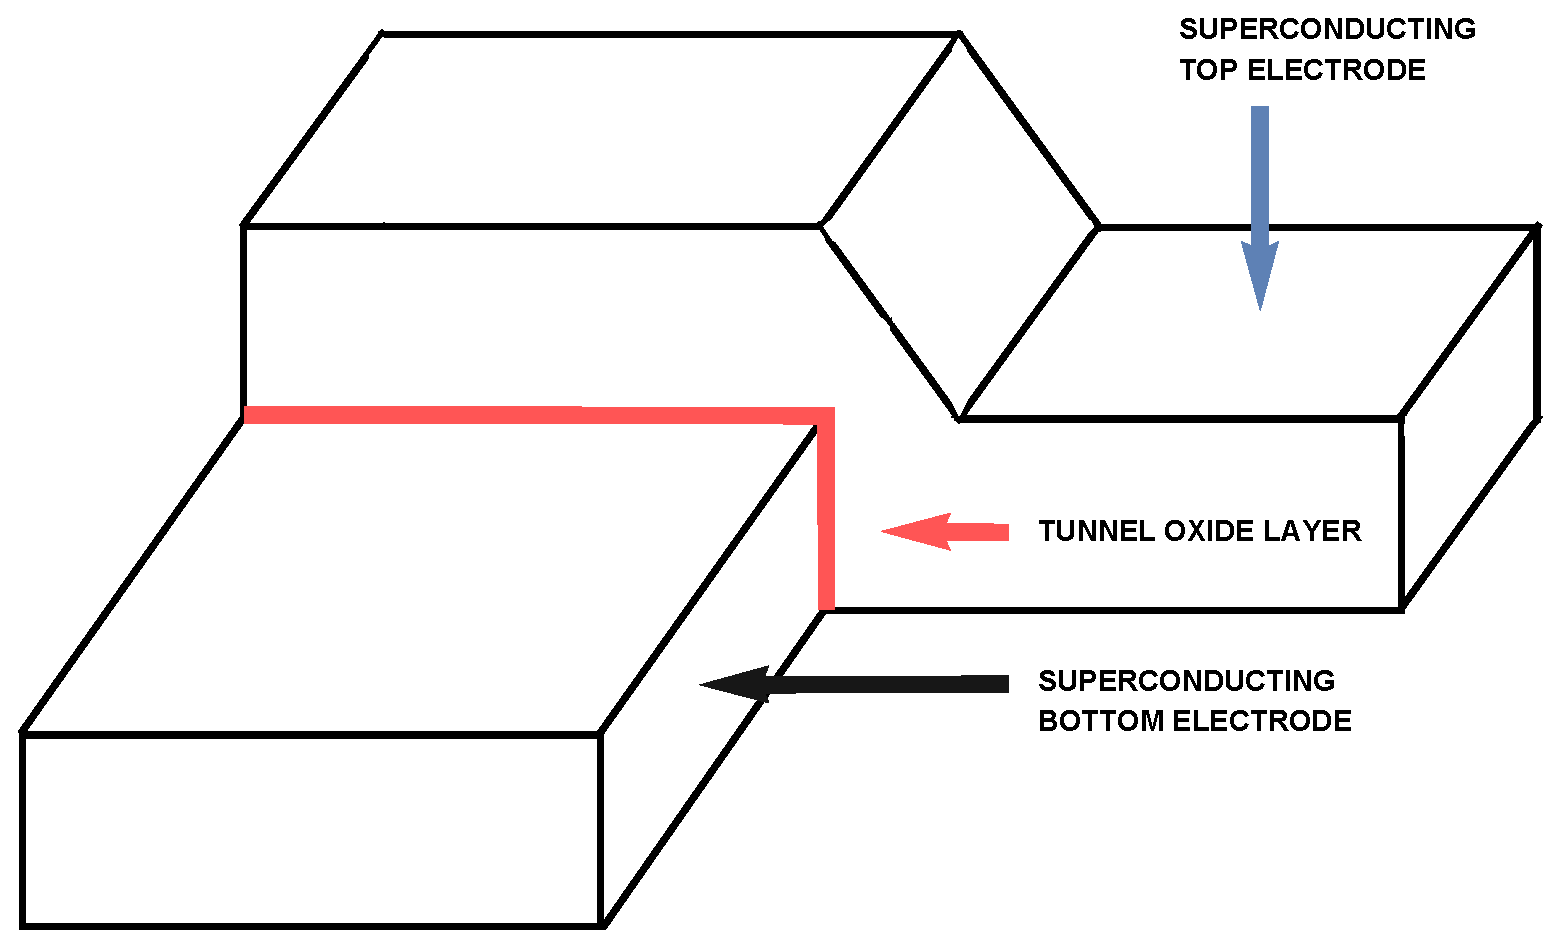
\includegraphics[width=0.8\textwidth]{./image/junction.eps}	}


	\end{columns}
	
		
 	\end{frame}


	\begin{frame}{Creare un circuito quantistico}

	\begin{figure} \includegraphics[width=0.95\textwidth]{./image/Circuito.png} \caption{Esempio circuito quantistico in Cirq. } \end{figure}
	
	\end{frame}
	
	\begin{frame}{Eseguire un circuito quantistico}
	
	Cosa significa eseguire un circuito? 
	\vspace{0.3cm}
	
	\begin{itemize}
	\item In una singola esecuzione con $n$ misure, il risultato sarà uno delle $2^n$ possibili stringhe binarie di $n$-bit. 
	\item Se l'esperimento è eseguito una seconda volta, anche se la misura è perfetta e non ha errori, il risultato potrebbe essere differente, compatibilmente con la casualità della 	meccanica quantistica. 
	\end{itemize}

	\vspace{0.3cm}
		
	\begin{columns}
	
	\column{0.7\textwidth}
	
	\vspace{-0.3cm}
	Quindi, il risultato di un circuito quantistico eseguito più volte, può essere rappresentato come una distribuzione su tutti i \alert{$2^n$ possibili risultati}, che possono essere illustrati in un istrogramma. 
		
	\column{0.3\textwidth}
	
	\vspace{-0.3cm}
	\centering \includegraphics[width=1\textwidth]{./image/Cirq_GHZ_Histogram.png} 


	\end{columns}

	
	\end{frame}


\backupend


%\begin{equation*}
%p = 1 - e^{-\Delta t / T} \quad \Longrightarrow \quad T= -\frac{\Delta t}{\log{(1-p)}}
% \end{equation*}



	
\end{document}
